\documentclass[
reprint,
amsmath,amssymb,showpacs,
aps,citeautoscript,prb,
onecolumn,notitlepage
]{revtex4-1}

\usepackage{graphicx}% Include figure files
\usepackage{bm}% bold math
\usepackage{float}
\usepackage{epstopdf}
\usepackage{tikz}
\usepackage{setspace}
\usepackage{physics}
% \usepackage{lipsum}
% \usepackage{babel}
\renewcommand{\l}{\langle}
\renewcommand{\r}{\rangle}
\begin{document}

\preprint{APS/123-QED}

\title{Title Goes Here}

\author{Evan Bluhm}
 
% \affiliation{
%  Physics Department, University of North Carolina at Chapel Hill
% }
\noaffiliation
\date{\today}

% \begin{abstract}

% \end{abstract}

\maketitle
\setstretch{1.5}

Example paragraph. Citations look like this \cite{Lamb01}. Math looks like this $1 + 2 = \alpha$. 

Equations look like this
\begin{equation}
\nabla ^2 \psi = 0
\end{equation}

And of course figures look like this

\begin{figure}[H]
\centering
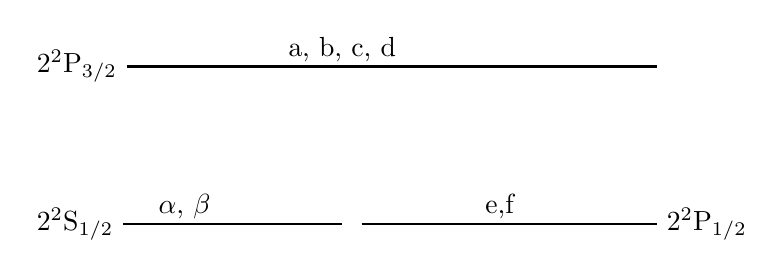
\begin{tikzpicture}[scale=1.0]
\node[anchor = west] at (-4,0) (l1) {2$^2$S$_{1/2}$};
\node[anchor=west] at (-0,0) (r1) {};
\node[anchor=west] at (0,0) (l2) {};
\node[anchor=west] at (4,0) (r2) {2$^2$P$_{1/2}$};
\node[anchor=west] at (-4,2) (l3) {2$^2$P$_{3/2}$};
\node[anchor=west] at (4,2) (r3) {};
\node[anchor=north] at (0,2.5) (a) {a, b, c, d};
\node[anchor=north] at (-2,0.5) (b) {$\alpha$, $\beta$};
\node[anchor=north] at (2,0.5) (c) {e,f};
\draw[thick] (l1) -- (r1);
\draw[thick] (r1) -- (r2);
\draw[thick] (l3) -- (r3);
\end{tikzpicture}
\caption{Fine structure of the  n = 2 levels of hydrogen.  According to the Dirac theory, the $2S_{1/2}$ and $2P_{1/2}$ levels are exactly degenerate.  The indices a, b, c, d, e, f, $\alpha$, $\beta$ denote the energetically degenerate magnetic sublevels.}
\label{fig:levels}
\end{figure}

Easy enough to refer to a figure like Figure \ref{fig:levels}

A much simpler figure looks like

\begin{figure}[H]
    \begin{center}
        \includegraphics[width=0.7\textwidth]{lambsetup.png}
    \end{center}
\end{figure}

I guess a quotation block might be nice?

\begin{quotation}
Hello, Zuko here. But I guess you probably already know me, sort of. Uh so, the thing is I have a lot of Firebending experience and I'm considered to be pretty good at it. Well you've seen me... you know when I was attacking you? Uh yeah, I guess I should apologize for that, but anyway I'm good now. I mean, I thought I was good before but now I realize I was bad, but anyway... I think it's time I joined your group and taught the Avatar Firebending.
\end{quotation}

\setstretch{1.0}
\nocite{*}
\bibliography{paper}% Produces the bibliography via BibTeX.

\end{document}
%
% ****** End of file apssamp.tex ******
